\chapter{Control Theory (linear): COMING SOON}
\label{ch-control-th}

\section{classical SISO model}

\begin{figure}[h!]
$$
\begin{array}{ccc}
\xymatrix{
\ar[d]^{r(t)}
\\
*+[F]{\sum}
\ar@{-}[d]^{+}
&\ar@{-}[l]^{-}_{f(t)}
\\
*+[F]{\stackrel{\rm Controller}{C}}
\ar@{-}[d]^{u(t)}
&
*+[F]{\stackrel{\rm Filter} {F}}
\ar@{-}[u]\ar@{-}[d]
&
\\
*+[F]{\stackrel{\rm Prossess} {P}}
\ar@{-}[r]^{y(t)}
&\ar@{-}[u]
}
\xymatrix{
\rvf(t_{k})\ar@/_1.5pc/[dd]
&
\rvf(t_{k+1})\ar@/_1.5pc/[dd]
\\
\rvr(t_{k})\ar[d]
&
\rvr(t_{k+1})\ar[d]
\\
\ul{\sum}(t_{k})\ar[d]
&
\ul{\sum}(t_{k+1})\ar[d]
\\
\rvu(t_{k})\ar[d]\ar[rd]
&\rvu(t_{k+1})\ar[d]
\\
\rvy(t_{k})\ar[r]\ar[ruuuu]
&
\rvy(t_{k+1})
}
\quad\quad\quad&
\xymatrix{
\rvf(t)\ar@/_1.5pc/[dd]
\\
\rvr(t)\ar[d]
\\
\ul{\sum}(t)\ar[d]
\\
\rvu(t)\ar[d]\ar@{~>}@/_1pc/[d]
\\
\rvy(t)\ar@{~>}@/_2pc/[uuuu]
\ar@(ur,dr)@{~>}[]
}
\end{array}
$$
\caption{xx}
\label{fig-siso}
\end{figure}





$t_k=t$, $t_{k+1}=t + \Delta t$, $\Delta t\rarrow 0$

\beq\color{blue}
P(r(t)) = given
\eeq

\beq\color{blue}
P(e(t+\Delta t)|
r(\cdot+\Delta t), f(\cdot))=
\delta(\quad
e(t+\Delta t)- [r(t+\Delta t)-f(t)]
\quad)
\eeq

\beq\color{blue}
P(u(t)|e(\cdot))=
\delta(\quad
u(t)-C[e](t)
\quad)
\eeq

\beq\color{blue}
P(y(t)|u(\cdot))
=\delta(\quad
y(t)-P[u](t)
\quad)
\eeq

\beq\color{blue}
P(f(t)|y(\cdot))
=\delta(\quad
f(t)-P[y](t)
\quad)
\eeq



\beq
\left\{
\begin{array}{l}
y(t) = (P\circledast  u)(t)
\\
u(t) = (C\circledast  e)(t)
\\
e(t)= r(t) - (F\circledast  y)(t)
\end{array}
\right.
\eeq

\beq
\left\{
\begin{array}{l}
\TIL{y}(s) = \TIL{P}(s)\TIL{u}(s)
\\
\TIL{u}(s) = \TIL{C}(s)\TIL{e}(s)
\\
\TIL{e}(s)= \TIL{r}(s) - \TIL{F}(s)\TIL{y}(s)
\end{array}
\right.
\eeq

\beq
\TIL{y}=\TIL{P}\TIL{C}[\TIL{r}-
\TIL{F}\TIL{y}]
\eeq

\beq
[1+\TIL{P}\TIL{C}\TIL{F}]\TIL{y}
=
\TIL{P}\TIL{C}\TIL{r}
\eeq

\beq
\TIL{y}=
\underbrace{
\left(
\frac{\TIL{P}\TIL{C}}
{1 + \TIL{P}\TIL{C}\TIL{F}}
\right)
}_{\TIL{H}(s)}
\TIL{r}
\eeq

PID (Proportional-Integral-Derivative) Controller

\beq
u(t)=
K_P e(t)
+K_I
\int_0^t
d\tau \;
e(\tau)
+
K_D\partial_t e(t)
\eeq


\beqa
\TIL{u}(s)
&=&
K_P\TIL{e}(s)
+ K_I \frac{\TIL{e}}{s}
+
K_D (s\TIL{e}(s)-
e(0^+))
\\
&=&
\underbrace{
\left(
K_P + \frac{K_I}{s}
+ K_D s
\right)
}_{\TIL{C}(s)}
\TIL{e}(s)
\quad\text{(assume $e(0^+)=0$)}
\eeqa

\beq
K_P = 2K,\;
K_D=KT,\; K=\frac{K}{T}
\eeq

\beq
\TIL{P}(s)= \frac{1}{K(1+sT)}
\eeq

\beq
\TIL{F}(s) = \frac{1}{1+sT}
\eeq



\beqa
\TIL{C}
&=&\frac{K}{sT}\left(2sT +1 + (sT)^2\right)
\\
&=&
\frac{K}{sT}\left(1 +sT\right)^2
\eeqa

\beqa
1+\TIL{P}\TIL{C}\TIL{F}&=&
1+\frac{1}{sT}
\\
&=&\frac{1}{sT}(1+sT)
\\
&=&
\TIL{P}\TIL{C}
\eeqa

\beq
\TIL{H}(s)=1
\eeq

\section{MIMO}



\section{Laplace Transforms}

This section
is a watered down version
of the Wikipedia entry 
for
Laplace Transforms
(Ref.\cite{wiki-laplace-transform}), which we highly recommend.

Let $0^- = 0-\eps$,
$0^+=0+\eps$
for some $\eps\in \RR$
such that $0<\eps<<1$.

Let $s=\s + i\omega$
for $\s,\omega\in\RR$.
$\s$ is called
the {\bf decay 
constant}
and $\omega$
is called the
{\bf angular frequency})

The {\bf Laplace Transform (LT)} of $f:[0,\infty]\rarrow \CC$
is defined as
\beq 
\call[f](s)=\TIL{f}(s)=
\int_{0-}^\infty dt\; e^{-st} f(t)
\label{eq-def-lap-trans}
\eeq
For LTs,
we assume functions 
$f(t)$ that
vanish for $t<0^-$.
They can jump
to a finite (with a step function) or
infinite value 
(
with a Dirac delta function) 
at $t=0$, 
but must vanish for $t<0^-$.
LTs are ideally
suited for solving
ordinary
differential
equations
with {\bf initial conditions}
such as $x(0)=5$, $\dot{x}(0)=10$.

The following
intuition
about LTs might
be helpful to th reader.
A LT is like 
a dot product of two vectors,
$e^{-st}$ and $f(t)$,
except that
in this case
the index $t$ for
their components
is a non-countable set $[0,\infty)$.
As with all
dot products, its maximum
is achieved 
if the two vectors 
point in the same
direction (this is
what the Cauchy Schwartz
inequality 
$\vec{a}.\vec{b}=
|\vec{a}||\vec{b}|\cos\theta
\leq |\vec{a}||\vec{b}|$
says).
In this case, if we substitute
$f(t) =\TIL{f}(s_0)e^{s_0t}$
on the right hand side
of Eq.(\ref{eq-def-lap-trans}),
we get  

\beqa
\TIL{f}(s)
&=&
\TIL{f}(s_0)
\int_{0^-}^\infty
dt\; e^{-(s-s_0)t}
\\
&=&
\TIL{f}(s_0)\delta(s-s_0)
\eeqa
So our intuition
is this:
whenever you see
an equation
involving LTs, 
replace each $f(t)$
by the special case
$f(t)= e^{s_ot}\TIL{f}$
(this is called a {\bf phasor}
when $s_0 = i\omega_0$),
and convince
yourself that
that the equation
is valid 
in the special case of phasors.


If the function $f(t)$
does not vanish for $t<0$,
we can use the
{\bf Bi-Laplacian Transform}
which is defined by
\beq
\calb[f](s)=
\int_{-\infty}^\infty
dt\; e^{-st} f(t)
\eeq
The Bi-Laplacian 
transform gives the
{\bf Fourier transform} when 
$s=i\omega$.
In this section,
we will only discuss the LT.


The {\bf Inverse
Laplace Transform}
is defined so that

\beq \call^{-1}[\underbrace{\call[f]}_{\TIL{f}}](t)
= f(t)
\eeq



If $f(t)=P(t)$
is a probability
distribution,
the LT 
is identical
to the 
{\bf Moment Generating function} in Probability Theory
\beq
\call[P](s)= E_\rvt[e^{-s\rvt}]
\eeq
The moments
generating function
can be used 
to calculate 
the moments of $\rvs$ as follows:
\beq
\av{s^n} = (-\partial_\rvs)^n E_\rvt[e^{-s\rvt}]
\eeq

Next, we 
will list
some of the
many
properties of 
LTs.
Henceforth,
we will
use the following
notation:

$a, b\in\CC$

$f,g:[0,\infty]\rarrow \CC$

$f(t)\maparrow{\call} \TIL{f}(s)$


\begin{itemize}

\item linearity

\beq
af(t)+bg(t)
\maparrow{\call}
a\TIL{f}(s)
+ b\TIL{g}(s)
\eeq

\item
Dirac delta function

\beq
\delta(t-a)
\maparrow{\call}
e^{-sa}
\eeq

\item 
Heaviside step function

Define the
{\bf Heaviside step function} by

\beq
step_a(t)=
\indi(t-a>0)
\eeq

\beq
step_a(t)
\maparrow{\call}
\frac{1}{s}
e^{-sa}\quad (for Re(s)>0)
\eeq

\item rectangular impulse

\beq
step_0(t) - step_a(t)
\maparrow{\call} \frac{1}{s}
(1-e^{-sa})\quad(for Re(s)>0)
\eeq

\item ramp

\beq
t\;step_0(t)
\maparrow{\call}
\frac{1}{s^2}
\quad(for Re(s)>0)
\eeq

\item sine, cosine

\beq
\sin(at)step_0(t) \maparrow{\call}
\frac{a}{s^2+a^2}
\eeq

\beq
\cos(at)step_0(t) \maparrow{\call}
\frac{s}{s^2+a^2}
\eeq

\item
polynomial rise, exponential drop

\beq
\frac{t^n}{n!}e^{-at}\;step_0(t)
\maparrow{\call}
\frac{1}{(s+a)^{n+1}}
\quad(for Re(s)>-a)
\eeq

\item Exponential approach to steady state

\beq
(1-e^{-at})step_0(t)
\maparrow{\call}
\frac{a}{s(s+a)}
\quad (for Re(s)>0, Re(s)>-a)
\eeq



\item Taylor series of $f(t)$

\beq
\int_0^\infty
dx\;e^{ -x} \frac{x^n}{n!}
=1
\eeq

\beq
\int_0^\infty dt\;e^{-st} \frac{t^n}{n!}
=\frac{1}{s^{n+1}}
\eeq

\beq
\frac{t^n}{n!}step_0(t)
\maparrow{\call}\frac{1}{s^{n+1}}
\eeq

\beqa
f(t)step_0(t)&=&
step_0(t)
\sum_{n=0}^\infty
\frac{t^n}
{n!}\partial_t^n f(0)
\\
&\maparrow{\call}&
\sum_{n=0}^\infty \frac{1}{s^{n+1}}
\partial_t^n f(0)
\eeqa

\item limits of $f(t)$


\beqa
\lim_{s\rarrow \infty}s\TIL{f}(s)
&=&
\lim_{s\rarrow \infty}s\int_0^\infty dt\; e^{-st}f(t)
\\
&\approx& 
f(0^+)\lim_{s\rarrow \infty}
\underbrace{s\int_0^\infty dt\; e^{-st}
}_{=1}
\\
&=&
f(0^+)
\eeqa

\beq
\lim_{s\rarrow 0}s\TIL{f}(s)
= f(\infty)
\eeq



\item convolution $(f\circledast  g)(t)$

The convolution
of $f:\RR\rarrow\CC$
and $g:\RR\rarrow\CC$
is defined by
\beq
(f\circledast  g)(t) = \int_{-\infty}^\infty
d\tau\; f(\tau)g(t-\tau)
\eeq
If $f(t)=g(t)=0$
for $t<0$,

\beq
(f\circledast  g)(t) = \int_{0}^t
d\tau\; f(\tau)g(t-\tau)
\quad
\text{(see Fig.\ref{fig-convolution}.)}
\label{eq-conv-left-half-zero}
\eeq

\begin{figure}[h!]
\centering
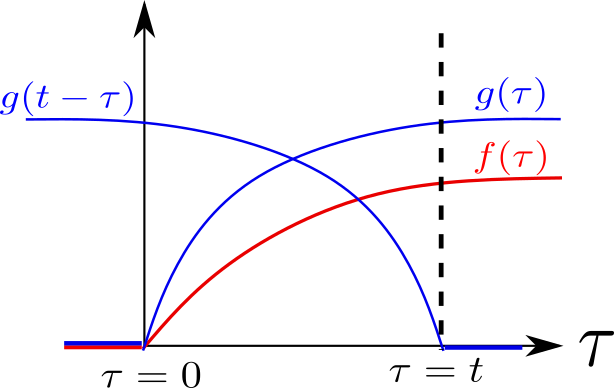
\includegraphics[width=3in]
{control-th/convolution.png}
\caption{Pictorial
representation
of the convolution
$(f\circledast g)(t)$. }
\label{fig-convolution}
\end{figure}

It's not hard to show that

\beq
f\circledast g = g\circledast f
\eeq
and that

\beq
(f\circledast  g)(t) \maparrow{\call}\TIL{f}(s)\TIL{g}(s)
\label{eq-lt-conv}
\eeq
Eq.(\ref{eq-lt-conv})
is easy to check
with phasors.
Indeed, if we substitute
$f(\tau)=e^{i\omega_0\tau}\TIL{f}$
and
$g(t-\tau)=
e^{i\omega_0(t-\tau)}\TIL{g}$,
on the right hand side
of Eq.(\ref{eq-conv-left-half-zero}),
the right
hand side
becomes $e^{i\omega_0t}\TIL{f}
\TIL{g}$,
and the LT of that
is $\TIL{f}
\TIL{g}$.




\item shifting $\TIL{f}(s)$ (frequency shifting)



\beq
e^{at}f(t)\maparrow{\call} \TIL{f}(s-a)
\quad\text{(for  $a>0$)}
\eeq



\item shifting $f(t)$ (time shifting).



\beq
f(t-a)\;step_a(t)\maparrow{\call}
e^{-as}\TIL{f}(s)
\quad\text{(for  $a>0$)}
\eeq

\item time scaling

\beq
f(at)
\maparrow{\call}
\frac{1}{a}
\TIL{f}
\left(\frac{s}{a}\right)
\quad\text{(for  $a>0$)}
\eeq


\item complex 
conjugation
\beq
f^*(t)\maparrow{\call}\TIL{f}^*(s^*)
\eeq

\item
derivatives of $\TIL{f}(s)$

\beq
(-t)f(t)
\maparrow{\call}
 \partial_s
\TIL{f}(s)
\eeq

\beq
(-t)^kf(t)
\maparrow{\call} (\partial_s)^k
\TIL{f}(s)
\eeq

\item
derivatives of $f(t)$

Define

\beq
f^{\geq 1}(t)
=f(t) - 
f(0^+)
\eeq


\beq
f^{\geq 2}(t)
=f(t) - 
f(0^+) - t f'(0^+)
\eeq

\beq
\partial_t f(t)
\maparrow{\call}
s
\TIL{f^{\geq 1}}(s)
\eeq


\beq
(\partial_t)^2 f(t)
\maparrow{\call}
s^2
\TIL{f^{\geq 2}}(s)
\eeq

\item
integral of $f(t)$

\beq 
\int_0^t d\tau\; f(\tau)
\maparrow{\call}
\frac{1}{s}\TIL{f}(s)
\eeq
Note that

\beqa
\int_0^t d\tau\; f(\tau)
&=&
\int_{-\infty}^\infty d\tau\; f(\tau)
step_0(\tau)step_0(t-\tau)
\\
&=&
((f step_0)\circledast  step_0)(t)
\eeqa


\item
integral of $\TIL{f}(s)$

\beq \frac{1}{t}f(t)
\maparrow{\call}
\int_s^\infty d\s\; \TIL{f}(\s)
\eeq

\item $f(t)$ periodic $f(t)=f(t+T)$

\beq
\cali_a^b=
\int_a^b dt\;
e^{-st}f(t)
\eeq

\beqa
\TIL{f}(s)
&=& \cali_0^T + \cali_{T}^{2T}
+
\cali_{2T}^{3T}+\cdots
\\
&=&
\cali_0^T(1 + e^{-sT} + e^{-s2T} +\cdots)
\\
&=&
\frac{1}{1-e^{-sT}}\cali_0^T
\eeqa

\beq
f(t)\maparrow{\call}
\frac{1}{1-e^{-sT}}
\int_0^T dt\;
e^{-st}f(t)
\eeq

\item Inverse LT

The inverse 
LT of a function
$\TIL{f}(s)$
can be calculated 
by performing
the
following
complex path integral:

\beq
\underbrace{\call^{-1}[\TIL{f}(s)](t)}_
{f(t)} = \frac{1}{2\pi i}
\lim_{T\rarrow \infty}
\int_{\gamma-iT}^{\gamma+iT}ds\;
e^{st}\TIL{f}(s)
\eeq
Another way of calculating
the inverse LT of $\TIL{f}(s)$, is
to express
$\TIL{f}(s)$ as a linear combination
of functions for which the inverse LT
is known from LT tables. For instance,

\begin{align}
\call^{-1}
\left[
\frac{1}{s(s-1)}
\right]
=&
\call^{-1}
\left[
\frac{1}{s} - \frac{1}{s+1}
\right] \text{(partial fractions expansion)}
\\
=&
\call^{-1}
\left[
\frac{1}{s}\right]
 - \call^{-1}
 \left[\frac{1}{s+1}\right]
 \\
 =&
 u_0(t)[1-e^{-t}]
\end{align}




\end{itemize}